% !TeX root = ../thuthesis-example.tex

\chapter{\MakeUppercase{NUIX-Studio Development kit}}

Дев кит используется разработчиками для создания новых устройств.
Он включает в себя:
1. Дизайнер устройств
2. api для поддержки сложных вычислений
3. api и инструменты для визуализации даты iot устройств
4. api для создания собственных виджетов

\section{Things Designer}

By using a block structure to represent devices, researchers can modify various parameters of existing devices by changing specific blocks and can create new devices by combining the blocks. This action is possible in a tool called Things designer. This tool is described in detail below.

The Semantic model is visualized inside the Web interface. Researchers can assign Widgets for each of the Items and group the Items together. After the setup is completed, researchers can further develop new devices inside the NUIX-Studio App. Next, they can create new Widgets in VR and connect them to the existing Items. The position for each of the Widgets is added to the Semantic model as an Item. Having set the Widget's position and other parameters, the user can exit the application on a device and then continue research using a different device or analyze the items' data stored on the server. Since changes in Items values are periodically written to the server, they can be visualized using the built-in system tools (Figure~\ref{fig:PersistenceExample-figure}) or further analyzed using external frameworks providing useful insights. The NUIX-Studio App also allows the creation of not only Widgets but also Items.

\begin{figure}
  \centering
  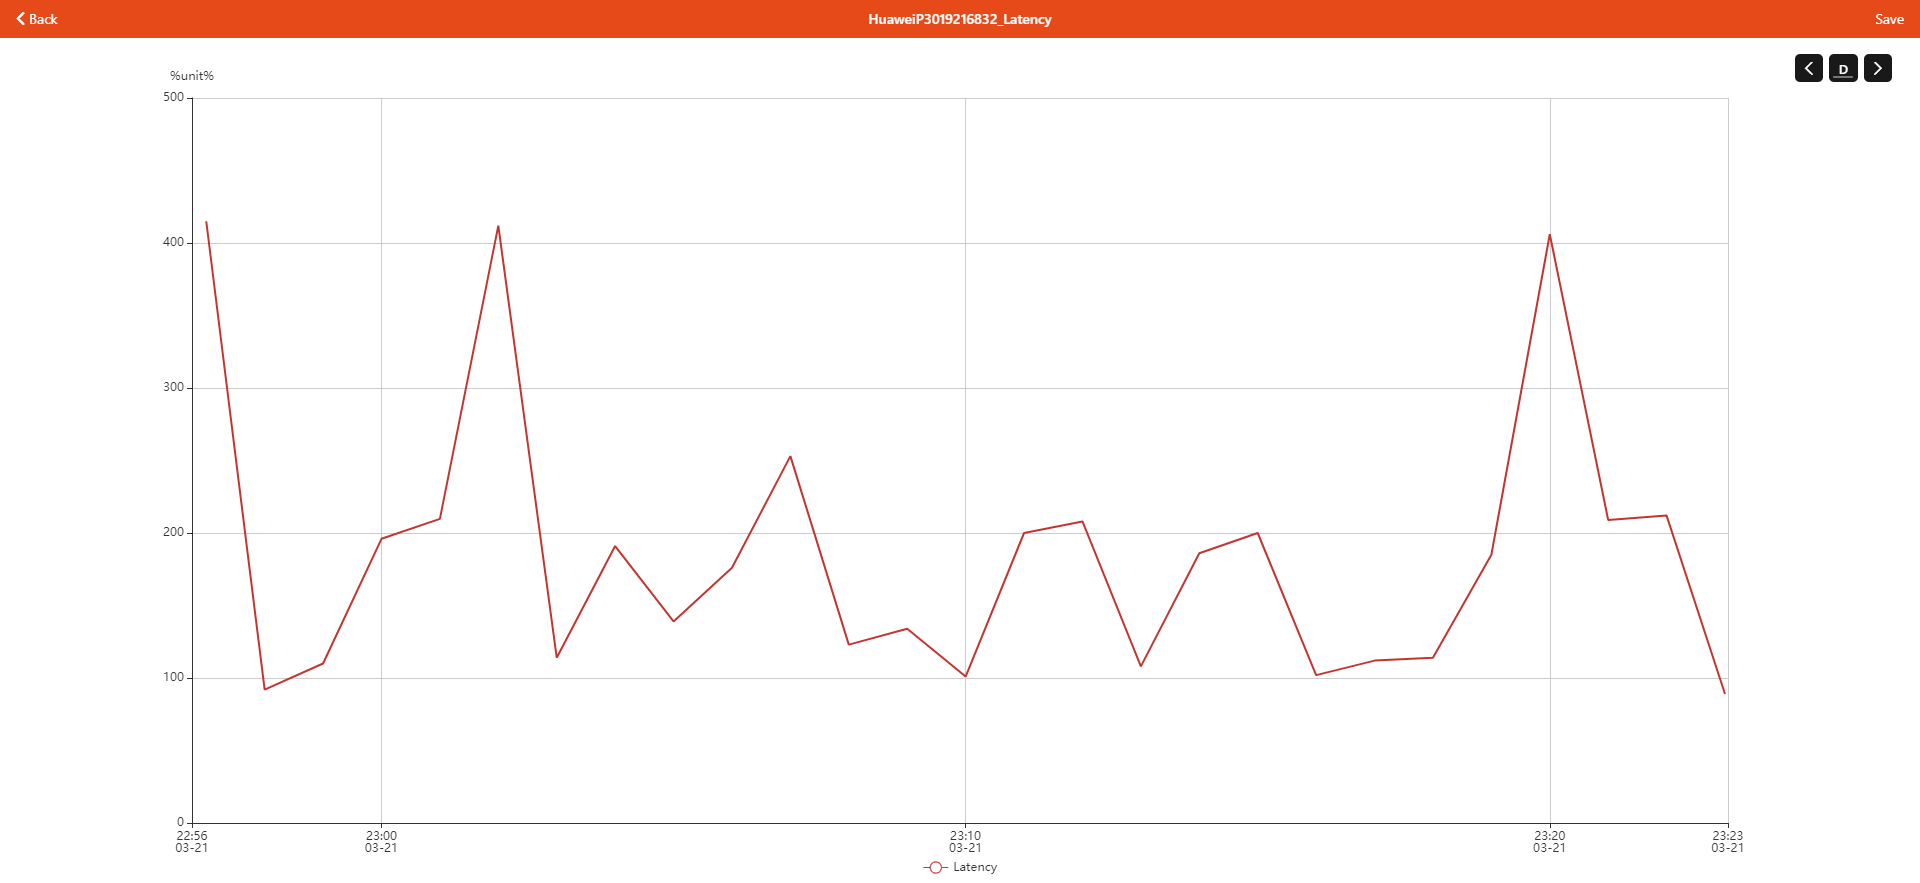
\includegraphics[width=0.9\linewidth]{figures/PersistenceExample.png}
  \caption{Persistence example: Latency value for accessing a remote device (in ms). }
  \label{fig:PersistenceExample-figure}
\end{figure}


\section{Performance-based calculations}

\subsection{Physics support}

With the transfer of resource-intensive calculations to a separate server, it becomes possible to perform more reliable physical object simulations. Computations such as processing light, sound, and electromagnetic waves of other frequencies and various substances such as gas, water, are only limited by existing algorithms.
\section{Device visualization and real-virtual world location mapping}

Each of the IoT devices is visualized through Widgets, but designing Widgets by 3D modeling requires additional time. If a 3D model of the device already exists, the researcher can add it to the platform as a Widget and then connect extra widgets to it.

In the IoT environment used, not every device has a corresponding 3D model. There are several solutions to this problem. The first solution is to use 3D models of similar devices. However, it is not always possible to find the particular model, or sometimes the quality of these models does not meet the requirements. The second solution is device scanning. With the help of 3D scanners based on depth cameras, it is already possible to scan things with acceptable accuracy and at a relatively affordable price. If millimeter precision scanning is required, then expensive professional solutions can be used.

The resulting Widgets of 3D models can be added to the Virtual reality. In the case of the NUIX-Studio App, scenes representing different environments are used. Scenes can be created within Unity editor and by using the Things designer, by interpreting the surrounding objects as Widgets (for example, people's position on the street is represented as an Item of Location type). This approach takes quite a long time to construct a scene, especially if one needs to use a copy of the real environment in Virtual reality. To reduce the time spent on 3D-modeling, researchers can use solutions such as 3D scanning of the environment. It is possible to scan the environment with good accuracy on many different smartphones using Depth Lab from Google and with excellent accuracy on the iPhone using Apple ARKit~\cite{baek_two-dimensional_2020, breitbarth_measurement_2019}. However, these scans of the environment are static scenes. If an object inside this environment is moved, then the scan will have to be performed again. Unfortunately, there is currently no solution to this problem. However, in the next chapter, it will be shown that the platform can be adapted to work with augmented reality, thus eliminating the need to match the real world with the virtual one fully.

Various devices can track the movement of real IoT devices in the real world, such as Bluetooth tags, QR codes, magnetic field sensors, etc. Researchers can use the API to change the position of each widget. Thus, when the device's position in the real world changes, the device's Widgets position in the virtual world will also change. It is also possible to perform the opposite action, but this requires a device that will move IoT devices in the real world.


\section{Widgets support}

The platform provides only basic Widgets for the Items. These Widgets are used to give an example of how to visualize the IoT devices' data. Researchers can create Widgets specific to the device they develop using the NUIX-Studio API.

However, in most cases, researchers can save time by using the basic Widgets. Several Widgets based on the Mixed Reality Toolkit, such as Color Picker, Pinch Slider, Switcher, and Button, were developed. Light-connection, Player-, Location- and Group-based Widgets were developed without using the Mixed Reality Toolkit.


\section{Summary}

убрать
убрать
убрать
убрать


Thus, it was shown that the platform's architecture supports all possible devices, creation of new devices from existing ones, and placing them in the virtual world. The platform enables the efficient processing of requests from an unlimited number of devices.

%However, the platform's architecture does not circumvent the limitations associated with some theoretical calculations. Yet, in order to get around these limitations, researchers can use the platform inside Augmented reality, which is discussed in more detail in the next chapter.

However, the platform's architecture does not circumvent the limitations associated with real-world technology restrictions, such as network latency. Implementation-based limitations are discussed in more detail in the next chapter.
